\chapter{\textit{Pipeline}}
\label{cha:pipeline}

\begin{figure}[!h]
\centering
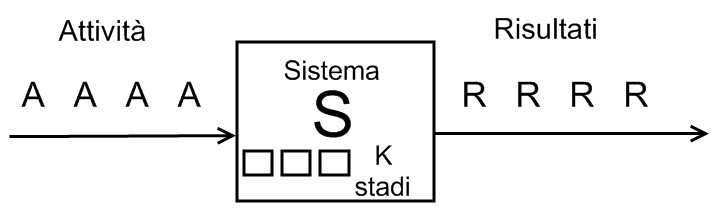
\includegraphics[width=0.5\columnwidth]{img/principioPipeline}
\caption{Schema di principio della \textit{pipeline}}
\label{fig:principioPipeline}
\end{figure}

Il \textit{pipelining} è oggi la principale tecnica di base impiegata per rendere performante una CPU. L'idea alla base del \textit{pipelining} è generale, e trova applicazione in molteplici settori dell'industria (linee di produzione, oleodotti, etc\ldots). Prendiamo in considerazione un generico sistema S che debba e eseguire alcune attività A (vedi fig. \ref{fig:principioPipeline}). Si chiama \textit{latenza (latency)} il tempo che intercorre fra l'inizio ed il completamento della generica attività A, mentre il \textit{throughput} è frequenza con cui vengono completate le attività.

Il \textit{pipelining} non riduce il tempo necessario al completamento di una singola attività, tuttavia incrementa il \textit{throughput} tante volte quanti sono gli stati della \textit{pipeline} (ma solo in un caso ideale!!).

\begin{figure}[!h]
\centering
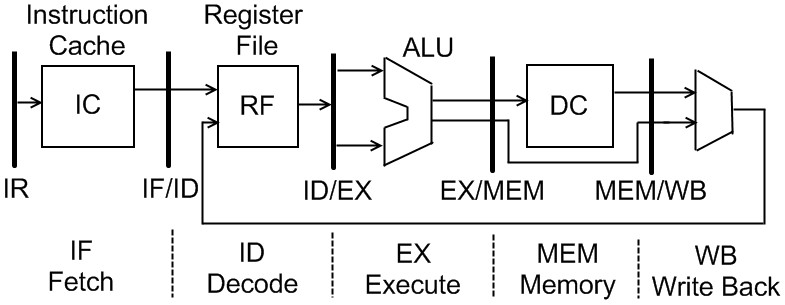
\includegraphics[width=0.7\columnwidth]{img/pipeline}
\caption{Struttura della \textit{pipeline} del DLX}
\label{fig:pipelineDLX}
\end{figure}

Nella \textit{pipeline} del DLX sono presenti cinque fasi principali (ogni fase rappresenta un particolare stadio, vedi fig. \ref{fig:pipelineDLX}):
\begin{itemize}
\item IF: \textit{Instruction Fetch}. Si legge in memoria qual è la prossima istruzione da eseguire;
\item ID: \textit{Instruction Decode}. Si leggono gli operandi sorgenti e si decodifica l'istruzione per capire cosa effettivamente dev'essere fatto;
\item EX: \textit{Execute}. In tale fase viene coinvolta la ALU e vengono effettuate le operazioni richieste dall'istruzione.
\item MEM: \textit{Memory Access}. Si memorizzano (eventualmente) i risultati della fase di EX.
\item WB: \textit{Write Back}. Si scrivono i risultati nel \textit{register file}\footnote{Memoria presente all'interno della CPU.}.

Purtroppo una \textit{pipeline} è suscettibile a stalli (vedi fig. \ref{fig:stallo}): gli stalli si generano quando si necessita di un dato che deve tuttavia ancora essere aggiornato con il suo corretto valore. Con gli stalli abbiamo quindi momenti in cui la CPU è bloccata (\textit{pipeline bloccante}) e impossibilitata ad eseguire nuove fasi delle varie istruzioni in quanto manca uno degli operandi: a causa di ciò, il $CPU_{time}$ della \textit{pipeline} non è pari al numero di istruzioni (come nel caso ideale), bensì pari a:
\[
CPU_{time} = 4 + N_{istruzioni}  + N_{stalli}
\]
Si noti che l'addendo $4$ si riferisce al numero di clock necessari a riempire la \textit{pipeline}. Risulta evidente che il numero di stalli influisce notevolmente sulle prestazioni: più stalliamo e più clock impieghiamo a completare una certa serie di operazioni. Infatti, se calcoliamo il cosiddetto CPI (\textit{Clock Per Instruction}) abbiamo:
\[
CPI_{medio}=\dfrac{4+N_{istruzioni}+N_{Stalli}}{N_{istruzioni}} ~~~
\mathop  \simeq \limits_{N_{Istruzioni} {\text{ alto}}} 
 ~~~
 1+\dfrac{N_{Stalli}}{N_{Istruzioni}}
\]

\begin{figure}[!h]
\centering
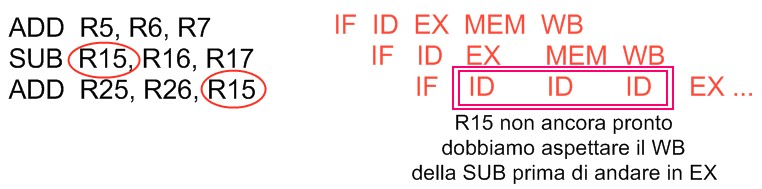
\includegraphics[width=0.8\columnwidth]{img/stallo}
\caption{Il meccanismo dello stallo}
\label{fig:stallo}
\end{figure}

\end{itemize}

\section{Miglioramenti alla \textit{pipeline}}
\label{sec:pipelineMiglioramenti}

Una possibile scelta per migliorare il funzionamento della \textit{pipeline} può essere quella di utilizzare più unità funzionali per ogni stadio (ad esempio più ALU). In tal caso si parla di \textit{macchina superscalare}.
Si può anche pensare di evitare lo stallo eseguendo, mentre un dato richiesto deve ancora aggiornarsi, un'istruzione successiva priva di \textit{alee} ("'dipendenze'"): questo accorgimento rende la pipeline\textit{ non bloccante}. 
Esempio:
\begin{verbatim}
ADD   R15, R16, R17
LD    R15, PIPPO(R16)
AND   R15, R16, R17
\end{verbatim}
Purtroppo qui non posso fare a meno di stallare, tuttavia posso eseguire eventuali istruzioni successive intanto che le tre illustrate vengono eseguite (OOO Execution, \textit{Out Of Order Execution}).

C'è inoltre da tener presente un aspetto importante: non tutti gli stadi vengono impegnati per un singolo clock. Istruzioni aritmetiche coi \textit{floating point} e/o altri tipi di operazioni piuttosto complesse possono richiedere, ad esempio, una permanenza nello stadio EX molto più duratura rispetto ad altre istruzioni.
Risulta quindi importante scoprire quale possa essere un buon metodo per rilevare possibili dipendenze, per risolvere le \textit{alee} e per individuare quindi le possibili situazioni di incoerenza fra i dati. Ad esempio, se prendiamo in considerazione le seguenti istruzioni
\begin{verbatim}
SUB   R15, R16, R17
AND   R25, R26, R15
\end{verbatim}
Questa dicitura è equivalente a:
\begin{verbatim}
R25 = R26 + (R16 - R17)
\end{verbatim} 
\begin{figure}[!h]
\centering
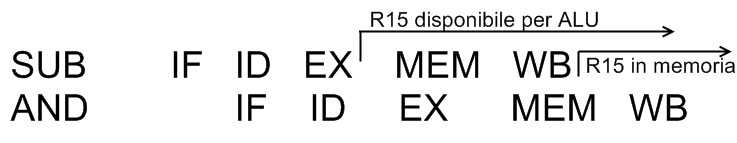
\includegraphics[width=0.7\columnwidth]{img/pipelineEsempio1}
\caption{}
\label{fig:pipelineEsempio1}
\end{figure}
In questo caso il risultato della SUB è necessario alla AND ma non vi sono alee se tali istruzioni vengono eseguite in sequenza (vedi fig. \ref{fig:pipelineEsempio1}): infatti è possibile retrazionare il registro EX-MEM verso la ALU (vedi fig. \ref{fig:retroazionamentoMux}).
\begin{figure}[!h]
\centering
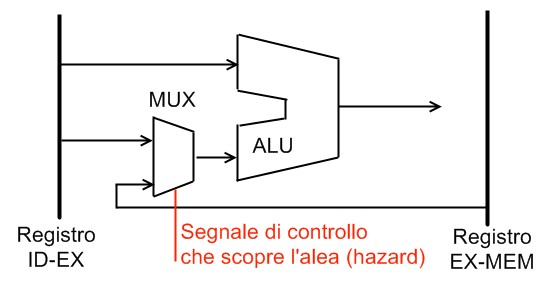
\includegraphics[width=0.6\columnwidth]{img/retroazionamentoMux}
\caption{Meccanismo di retroazione e segnale di controllo}
\label{fig:retroazionamentoMux}
\end{figure}
Risulta quindi necessaria una \textit{Hazard Detection Unit} per scoprire se ci sia l'alea o meno: essa deve gestire il segnale di controllo del MUX (vedi fig. \ref{fig:pipelineEsempio1}) bypassando il \textit{register file}\footnote{In caso contrario avremmo dovuto attendere la fase di WB.}. Questo permette di risparmiare notevoli clock altrimenti persi a causa di stalli.

\begin{figure}[!h]
\centering
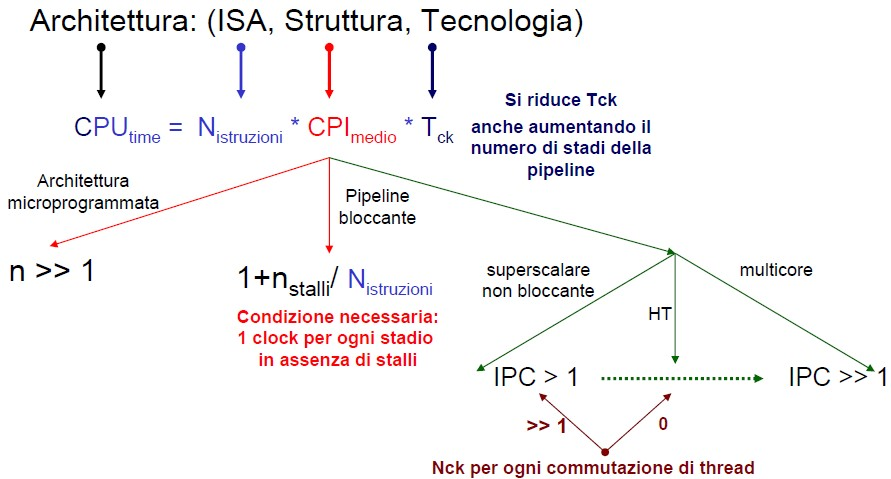
\includegraphics[width=\columnwidth]{img/schemaRiassuntivoArchitetture}
\caption{Schema riassuntivo delle scelte architetturali}
\label{fig:schemaRiassuntivoArchitetture}
\end{figure}

\section{\textit{Pipeline} con stadi a ciclo singolo}
\label{sec:pipelineStadiCicloSingolo}

Prendiamo in considerazione una \textit{pipeline} a ciclo singolo, come quella in figura \ref{fig:pipelineDLX}. Supponendo che il ritardo fra i diversi stadi sia pari a $t_{si}$ la frequenza di clock è vincolata dalla seguente relazione:
\[
t_{ck} \geq 
\mathop {\max }\limits_i \left( {t_{si}  + \underbrace {t_{CHOV\max } }_{{\text{CHOV  = }}{\text{ clock high out valid}}} + \underbrace {t_{SU\min } }_{{\text{SU  =  set up}}}} \right)
\]
In questa relazione
\begin{itemize}
\item $t_{CHOV\max}$ è il massimo ritardo dei registri prima che il dato sia valido in uscita;
\item $t_{SU\min}$ è il tempo di \textit{set-up} minimo (il dato deve rimanere costante).
\end{itemize}

E se volessimo andare più forte con la frequenza di clock (e quindi abbassare $t_{ck}$)? Abbiamo due possibilità d'azione:
\begin{enumerate}
\item Adottiamo una tecnologia migliore.
\item A parità di tecnologia poniamo dei registri all'interno di ogni stato (architettura \textit{Super-Pipelined}, vedi fig. \ref{fig:superpipeline}).
\end{enumerate}
\begin{figure}[!h]
\centering
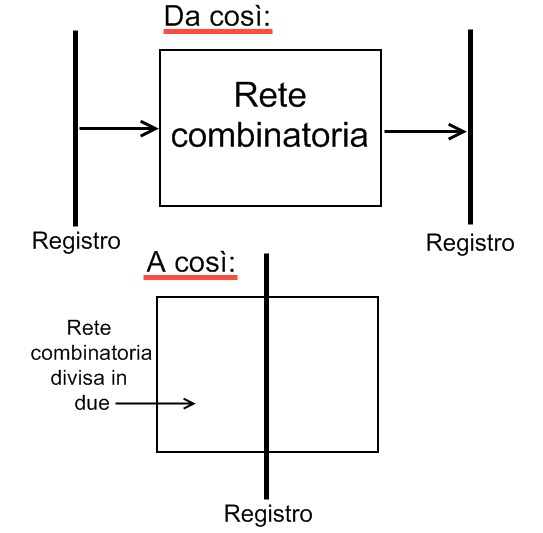
\includegraphics[width=0.5\columnwidth]{img/superpipeline}
\caption{Principio dell'architettura \textit{Super-Pipelined}}
\label{fig:superpipeline}
\end{figure}

\section{Alee}
\label{sec:alee}

\subsection{Alea strutturale}
\label{sec:aleaStrutturale}

Esistono operazioni (come la FDIV, FMUL o FADD, che agiscono su numeri \textit{float}) in grado di impegnare lo stadio EX per molti cicli di clock, compromettendo con reiterati stalli le prestazioni della macchina. Si parla, in questo caso, di \textit{alea strutturale}: a causa degli stalli indotti da tale tipo di alea, uno stadio impegnato per $n$ cicli è in grado di bloccare la \textit{pipeline} per $n-1$ periodi di clock (fino, cioè, al definitivo completamento del calcolo da effettuare). Molte alee strutturali possono quindi far drammaticamente crollare la velocità della nostra \textit{pipeline} con stadio a ciclo singolo mentre, viceversa, se esse non sussistessero sarebbe possibile effettuare molte più istruzioni. Supponendo ad esempio di dover fare 1 DIV (40 clock ciascuna), 10 FADD (4 clock ciascuna) e 40 AND (1 clock ciascuna), impiegheremmo $\{\max \left( {1 \cdot 40,10 \cdot 4,40 \cdot 1} \right)\} = 40$ clock contro i $40+10+1=51$ dei quali avremmo bisogno nel caso di unica unità funzionale: lo \textit{speed-up} della \textit{pipeline} multiciclo è quindi notevole. 

Per ridurre o eliminare gli stalli si può quindi scegliere di implementare \textit{pipeline} con più unità multiciclo in parallelo all'unità di esecuzione intera (vedi fig. \ref{fig:multicycle}). In questo modo è possibile effettuare operazioni diverse in parallelo, guadagnando notevolmente in prestazioni: 

\begin{figure}[!h]
\centering
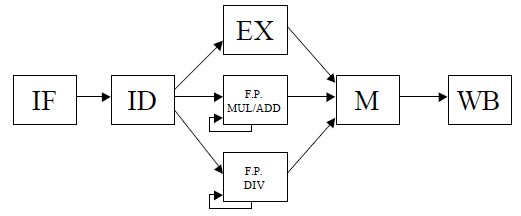
\includegraphics[width=0.55\columnwidth]{img/multicycle}
\caption{Pipeline del DLX con stadi \textit{multicyle} in parallelo}
\label{fig:multicycle}
\end{figure}

\begin{figure}[!h]
\centering
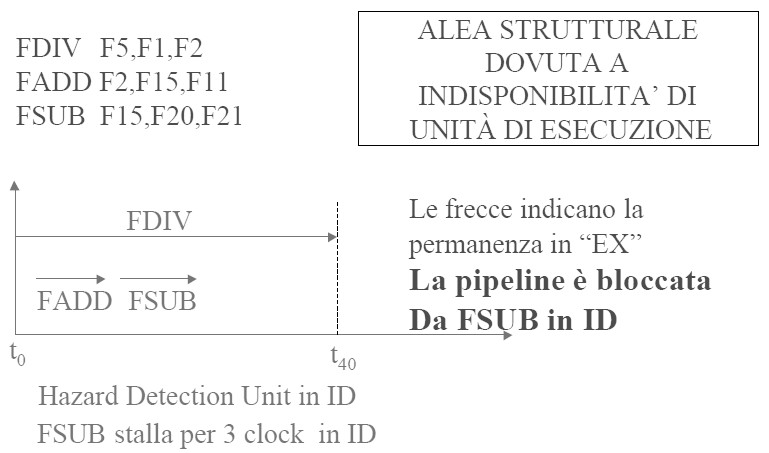
\includegraphics[width=0.7\columnwidth]{img/aleaStrutturale}
\caption{Meccanismo dell'alea strutturale}
\label{fig:aleaStrutturale}
\end{figure}

\subsection{Alea di dato, alee WAW, WAR, RAW}
\label{sec:aleaDato}

Di parla di \textit{alea di dato} (o \textit{alea RAW}, \textit{Read After Write}\footnote{Leggendo oltre si capirà anche il perché di questa denominazione: devo infatti leggere il nuovo dato dopo averlo scritto (calcolato).}) quando, per proseguire, si ha bisogno di un dato che sta per essere calcolato ma impiega molti clock costringendoci ad aspettare. Questo problema può essere parzialmente risolto con l'accelerazione apportata dalla \textit{pipeline multiciclo} (vedi par. \ref{sec:aleaStrutturale}), tuttavia è possibile fare anche di meglio: si può infatti ovviare al problema eseguendo le istruzioni fuori ordine (OOO = \textit{Out Of Order}), effettuando cioè istruzioni successive a quella che sarebbe obbligatorio fare se agissimo in maniera perfettamente sequenziale nel mentre il dato di cui abbiamo bisogno viene calcolato\footnote{"'Devo aspettare che mi arrivi il dato? Nel frattempo faccio altro, sennò starei lì ad oziare.'"}.

\begin{figure}[!h]
\centering
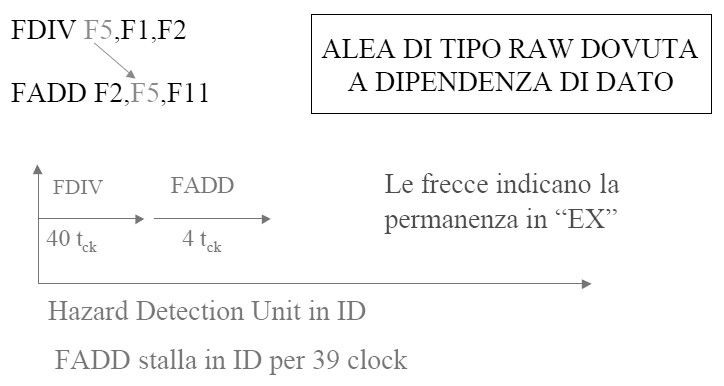
\includegraphics[width=0.7\columnwidth]{img/aleaDato}
\caption{Meccanismo dell'alea RAW (o di dato)}
\label{fig:aleaDato}
\end{figure}

Attenzione! Non si possono invertire le istruzioni a cuor leggero: si rischia infatti di cadere nello stesso errore dal quale cerchiamo di sfuggire, eseguendo cioè istruzioni non effettuabili avendo noi bisogno del dato aggiornato (che è in calcolo)! Il completamento fuori ordine può inoltre rendere imprecisa la gestione delle
eccezioni; ne consegue una esecuzione non corretta del codice, con possibilità di perdere informazioni in modo irrecuperabile. Da qui la necessità di un metodo per capire se sia possibile invertire l'esecuzione di due particolari operazioni, di una modalità - ovvero - di \emph{estrarre il parallelismo intrinseco del codice}\footnote{Ooooooohhh... :-o} \footnote{Detto anche ILP, \textit{Instruction Level Parallelism}.}: in soldoni, devo poter estrarre le dipendenze, le quali hanno tre modi di manifestarsi:
\begin{itemize}
\item \textbf{dipendenza di dato}: già vista poco sopra (par. \ref{sec:aleaDato});
\item \textbf{dipendenza di nome}: due istruzioni usano lo stesso registro ma senza passaggio di dati;
\item \textbf{dipendenza di controllo}: caso suddivisibile in \textit{antidipendenza}, che si verifica "'anticipando'" un'istruzione e rischiando quindi di scrivere su un registro coinvolto in un'operazione precedente, come nel seguente codice
\begin{verbatim}
FADD    F10, F5, F3
FDIV    F5, F1, F1
\end{verbatim}
e \textit{dipendenza d'uscita}, quando un registro contiene il risultato di due operazioni differenti, come accade nelle seguenti righe di assembler:
\begin{verbatim}
FADD    F5, F26, F3
FDIV    F5, F1, F1
\end{verbatim}

L'antidipendenza si manifesta nella cosiddetta alea \textit{Write After Read} (WAR), la quale comporta che il flusso nella \textit{pipeline} non possa proseguire in quanto si deve scrivere su un registro che una istruzione precedente deve leggere ma non ha ancora letto. Fortunatamente le alee WAR non sono possibili in quanto gli operandi
sono sempre letti in nella fase ID, quindi è impossibile che, quando si legge un operando, l'istruzione successiva
l'abbia già aggiornato.

La dipendenza d'uscita, invece, comporta l'alea \textit{Write After Write} (WAW), che si ha quando il flusso nella \textit{pipeline} non può proseguire in quanto una istruzione precedente deve ancora scrivere su un registro che anche
l'istruzione corrente deve aggiornare.
\begin{figure}[!h]
\centering
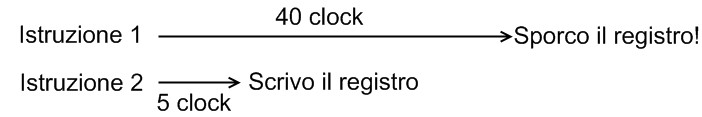
\includegraphics[width=0.7\columnwidth]{img/areaWAW}
\caption{L'alea WAW}
\label{fig:areaWAW}
\end{figure}
Come risolvere l'erronea scrittura di un registro (vedi fig. \ref{fig:areaWAW})? Possiamo pensare di intimare alla prima istruzione di non aggiornare F5 (in alcuni casi le alee WAW si possono eliminare inibendo il
completamento dell'istruzione che determina il malfunzionamento), potremmo effettuare qualche altra istruzione tra la prima e la seconda oppure, se proprio non abbiamo scelta, non ci rimarrà che stallare. In particolare, si dice che una \textit{pipeline} gestisce le eccezioni in modo preciso se essa può essere fermata in modo che tutte le istruzioni precedenti l'istruzione in cui l'eccezione si è verificata siano completate, mentre tutte le istruzioni successive non modifichino lo stato della CPU prima che l'eccezione sia stata servita.
\end{itemize}

In alcuni casi le alee possono rivelarsi davvero pervasive (vedi fig. \ref{fig:aleeABalusa}).
\begin{figure}[!h]
\centering
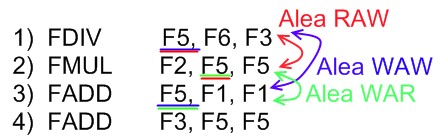
\includegraphics[width=0.5\columnwidth]{img/aleeABalusa}
\caption{Sequenza non indifferente di alee}
\label{fig:aleeABalusa}
\end{figure}
Per evitare situazioni erronee si effettua la fase di \textit{fetch} in sequenza e poi l'ordine viene stabilito dal microprocessore in base alle alee: il criterio è quello di eseguire le istruzioni nell'ordine in cui si hanno a disposizione gli operandi (modalità di tipo \textit{data flow}).
Questo comporta l'essere in grado di poter rinominare i registri (\textit{register renaming}) con valori temporanei (vedi fig. \ref{fig:aleeABalusa2}).
\begin{figure}[!h]
\centering
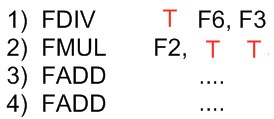
\includegraphics[width=0.3\columnwidth]{img/aleeABalusa2}
\caption{\textit{Register renaming}}
\label{fig:aleeABalusa2}
\end{figure}

\subsection{Alee di controllo}
\label{sec:aleeControllo}

Si hanno quando una delle istruzioni comporta il trasferimento di controllo.
Esempio:
\begin{verbatim}
BEQZ    R6, PIPPO
ADD     R6, R7, R8
\end{verbatim}
Queste istruzioni non possono essere eseguite in parallelo: prima va verificata la condizione, poi si calcola dove si deve saltare e infine si valuta se saltare oppure no. Una politica spesso adottata dai processori è quella di \textit{predire di non saltare}, ovvero supporre che non sarà necessario effettuare la \textit{branch}: questa scelta rientra nell'ambito della cosiddetta \textit{esecuzione speculativa} e comporta l'eseguire in maniera "'provvisoria'" istruzioni successive a quella del salto, per poi darle per buone in caso di corretta previsione oppure scartarle nel caso di predizione sbagliata (\textit{misprediction}).

\begin{figure}[!h]
\centering
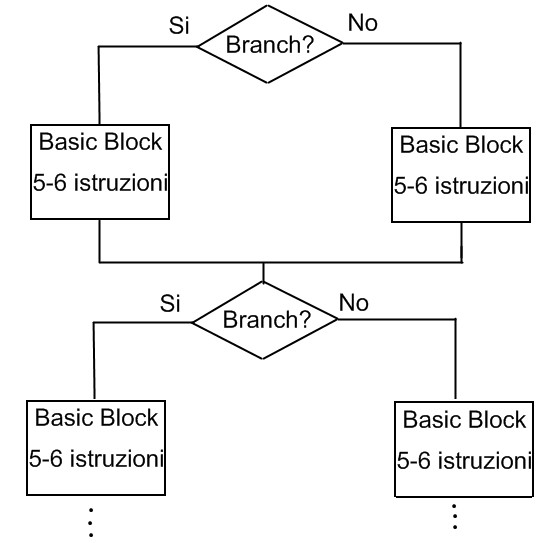
\includegraphics[width=0.5\columnwidth]{img/flowChartTipo}
\caption{Tipica \textit{flow chart} di un programma}
\label{fig:flowChartTipo}
\end{figure}

Statisticamente si è appurato che, tra \textit{branch} e \textit{branch}, vi sono sempre circa 5-6 istruzioni indipendenti (vedi fig. \ref{fig:flowChartTipo}). Nell'esecuzione speculativa, quindi viene in genere eseguito almeno un BB (\textit{basic block}) successivo dopo una \textit{branch}, validando ciò che si è fatto una volta che si è scoperto di aver evitato l'alea oppure annullando tutto in caso di \textit{misprediction} (qui torna utile l'abilità della CPU di poter fermare la \textit{pipeline} in modo che tutte le istruzioni precedenti la \textit{branch} siano completate e senza che le istruzioni successive abbiano effetto).

\section{L'approccio di Tomasulo}
\label{sec:tomasulo}

L'algoritmo di Tomasulo è un approccio di \textit{scheduling} dinamico per l'esecuzione delle istruzioni:
\begin{itemize}
\item consente di riconoscere situazioni di ILP non riconoscibili al tempo di compilazione;
\item riduce la complessità dei compilatori;
\item consente al codice compilato per una \textit{pipeline} di essere eseguito anche su \textit{pipeline} diverse;
\item rende molto più complesso l'hardware dell'unità di esecuzione.
\end{itemize}

In base ad esso, ogni unità di esecuzione \textit{multicycle} viene equipaggiata con stazioni di prenotazione (\textit{reservation stations}) che ospitano sia l'istruzione in esecuzione, sia istruzioni pronte per essere eseguite e in attesa dell'unità di esecuzione, sia istruzioni sospese in attesa di uno o due
operandi. Nello stadio ID l'istruzione viene decodificata e inviata a una appropriata \textit{reservation
station}, se disponibile; altrimenti, causa alea strutturale o mancanza di
\textit{reservation stations}, si stalla. 

\begin{figure}[!h]
\centering
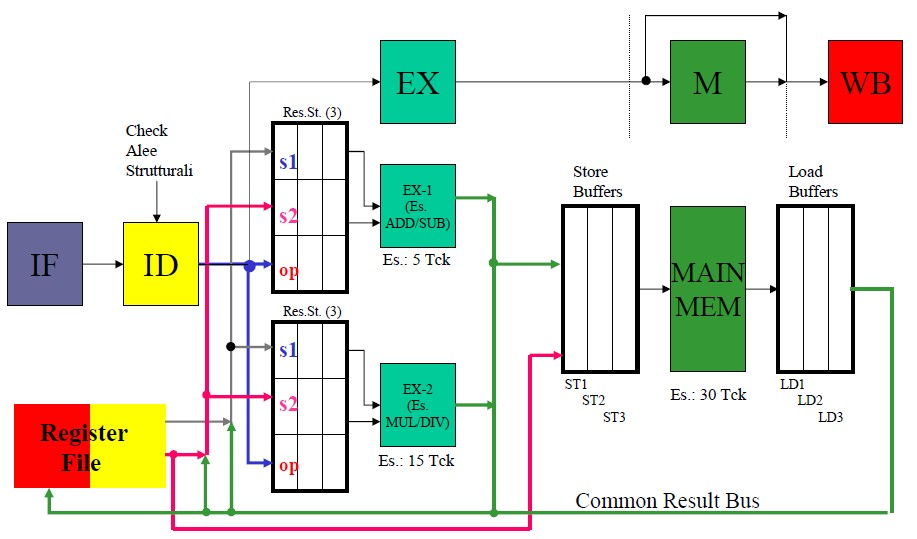
\includegraphics[width=0.9\columnwidth]{img/tomasulo}
\caption{Architettura prevista per il funzionamento dell'algoritmo di Tomasulo}
\label{fig:tomasulo}
\end{figure}

Alla \textit{reservation station} vengono inviati anche gli operandi, se disponibili; altrimenti si invia l'identificatore (\textit{tag}) della RS che fornirà l'operando mancante (nel caso dell'alea di dato). Il risultato generato dall'unità EX, insieme al \textit{tag} della RS che identifica l'operazione eseguita, viene messo a disposizione del \textit{register file} (in modo che possano usufruirne tutte le unità di EX che lo richiedono) e dello stadio MEM (attraverso il \textit{Common Result Bus}). Le alee RAW sono dunque risolte con il \textit{forwarding} (cioè l'invio) dei risultati a tutte le unità che hanno bisogno di operandi (\textit{reservation stations} e memorie).

\begin{figure}[!h]
\centering
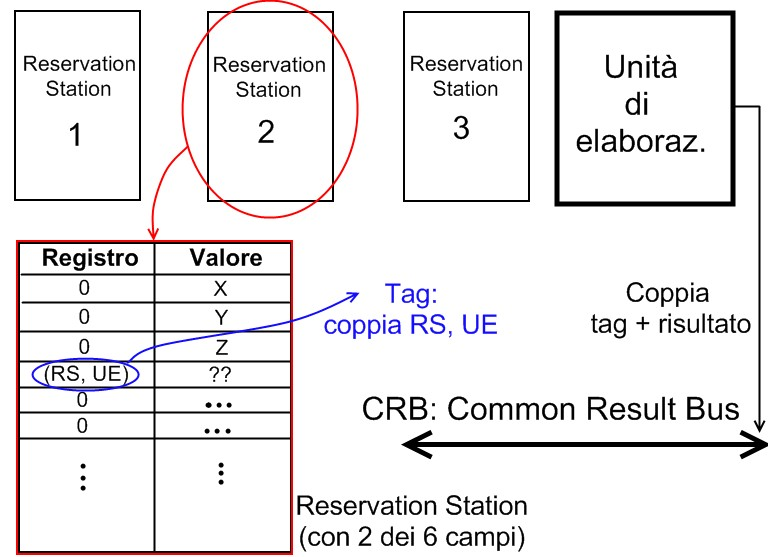
\includegraphics[width=0.75\columnwidth]{img/tomasulo2}
\caption{Architettura prevista per il funzionamento dell'algoritmo di Tomasulo (2)}
\label{fig:tomasulo2}
\end{figure}

Colui che ha bisogno di un risultato controllerà il CRB cercando in base al tag. Infatti, ad ogni unità che produce risultati (\textit{Load Buffer, Reservation Station}), è associato un identificatore che viaggerà sul \textit{Result Bus} insieme al risultato stesso.

Le \textit{reservation station} hanno 6 campi (in figura \ref{fig:tomasulo2} ne vengono illustrati solo 2):
\begin{itemize}
\item  BUSY: indica se la RS è libera o occupata
\item  $Q_j$ e $Q_k$: contengono l'identificatore del \textit{Load Buffer} o della \textit{Reservation
Station} che produrrà l'operando sorgente ($j$: 1° operando, $k$: 2° operando)
\item  $V_j$ e $V_k$: contengono l'operando se $Q_j$ / $Q_k$ = 0
\item  OP: operazione da eseguire (Es: FADD/FSUB\ldots)
\end{itemize}
\begin{figure}[!h]
\centering
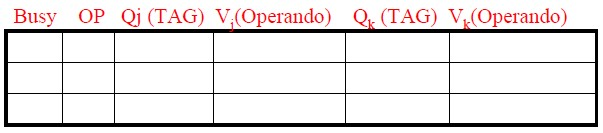
\includegraphics[width=0.75\columnwidth]{img/reservationStation}
\caption{I campi della \textit{reservation station}}
\label{fig:reservationStation}
\end{figure}

Poniamo ora di essere nella fase di ID (per ipotesi) di un'operazione DIV fra gli operandi OP1 e OP2. Abbiamo una \textit{reservation station} libera? Se sì la prenotiamo e, nel \textit{register file}, scriviamo la coppia (RS, UE): questo significa che il \textit{register file} aspetta il risultato dalla \textit{reservation station} RS appartenente all'unità operativa UE. Quando essa giunge alla fase di WB, viene scritto su CRB il risultato abbinato al relativo \textit{tag}: a quel punto il \textit{register file} si accorge che il risultato c'è è setta l'identificativo "'0'" (= dato disponibile, vedi campo \textit{registro} in fig. \ref{fig:tomasulo2}) presso il relativo operando. In questo modo deleghiamo la comunicazione del risultato alla \textit{reservation station}, utilizzando i \textit{tag} per suggerire cosa dovrà essere pescato dal \textit{common result bus}.

I registri posti prima del CRB (vedi fig. \ref{fig:tomasulo}) servono per evitare l'eventualità di due WB contemporanee (NOTA: la disponibilità di un operando si ha a partire dal termine della fase di WB): all'interno dello stesso ciclo di clock possiamo quindi scrivere più di un registro a monte del CRB, ma su quest'ultimo può essere scritto solo un dato alla volta.
Di conseguenza si ha che, con un solo CRB, non potremo effettuare più di un'operazione per clock ($CPI_{max} =1$); con più CRB è invece possibile completare più istruzioni simultaneamente (cioè in un singolo clock):
\[
N_{CRB} = N_{\text{Istruzioni simultaneamente completabili}}
\]
Nel caso di unico CRB e necessità di completare due istruzioni, è indifferente quale delle due scrivere per prima: negli esercizi si consiglia di scegliere una regola e agire coerentemente ad essa.

\section{Architettura protetta e Tomasulo}
\label{sec:protectedTomasulo}

Supponiamo di dover effettuare la seguente serie d'operazioni:
\begin{verbatim}
FDIV    F5, F1, F2
FADD    F20, F20, F21
FSUB    F5, F20, F12
\end{verbatim}
Se per caso F2 valesse zero avremmo un'operazione illegale (divisione per zero) e quindi verrebbe lanciata un'eccezione tramite un \textit{interrupt}, che fungerebbe da spartiacque fra le istruzioni precedenti e quelle successive. Se agissimo secondo una logica puramente sequenziale (\textit{In Order Issue}) saremmo costretti a stallare fino alla risoluzione dell'eccezione; se invece eseguissimo \textit{Out Of Order} dovremmo stare attenti a   non sporcare il valore dei registri completando istruzioni successive con operandi non aggiornati. Come abbiamo già detto, la politica è quella di salvare i risultati in un \textit{buffer} temporaneo e di farli diventare definitivi una volta che si è effettuato il controllo di \textit{safety}, cioè di sicurezza (correttezza). In effetti questa è una parte molto delicata per il funzionamento della nostra \textit{pipeline}: abbiamo accennato infatti alla possibilità di effettuare esecuzione speculativa, azzardando una predizione per un certo numero di istruzioni successive (dipendente dal numero di \textit{reservation station}), e abbiamo sottolineato l'importanza di poter annullare quanto supposto in caso di \textit{misprediction}. Quanto auspicato è ottenibile con Tomasulo se aggiungiamo una fase di \textit{Write Temporary} (WT, vedi fig. \ref{fig:safetyTomasulo}), durante la quale è il ROB (\textit{re-order buffer}, vedi fig. \ref{fig:safetyTomasulo2}) e non il \textit{register file} a mettere a disposizione i risultati.

\begin{figure}[!h]
\centering
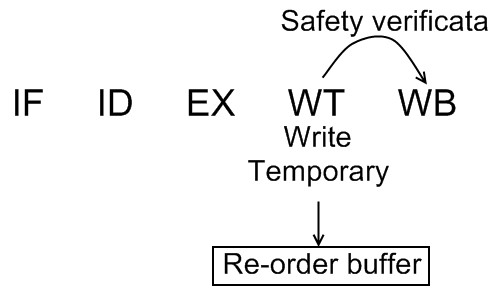
\includegraphics[width=0.5\columnwidth]{img/safetyTomasulo}
\caption{Miglioramento alla soluzione di Tomasulo}
\label{fig:safetyTomasulo}
\end{figure}

\begin{figure}[!h]
\centering
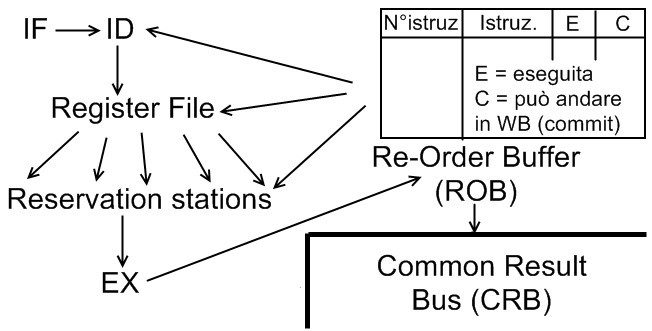
\includegraphics[width=0.65\columnwidth]{img/safetyTomasulo2}
\caption{Miglioramento alla soluzione di Tomasulo (2)}
\label{fig:safetyTomasulo2}
\end{figure}

Quando abbiamo predetto bene, nel ROB vengono posti degli 1 in prossimità delle istruzioni eseguite perché potevano effettivamente esserlo. Una volta che tale ambiguità è stata risolta, la parte completata viene svuotata dal ROB.
Pertanto, in questo nuova logica, il TAG non è più (RS, UE) ma l'indice nel ROB in cui è posta l'istruzione che deve restituirci il risultato.

Questo sistema è robustissimo con le alee RAW e, abbinato a una robusta logica di predizione (per evitare le alee di controllo in particolare), garantisce un'ottima protezione. 

\section{Protezione e memorie associative}
\label{sec:memorieAssociative}

Il problema dell'esecuzione speculativa richiede una nuova struttura dati per memorizzare i PC relativi ad una scelta di predizione rispetto che ad un altra (vedi fig. \ref{fig:plusFour}): una scelta funzionale e in grado di garantire velocità e affidabilità è quella che vede l'utilizzazione di una memoria associativa (nome/valore, detta CAM - \textit{Content Access Memory}).

\begin{figure}[!h]
\centering
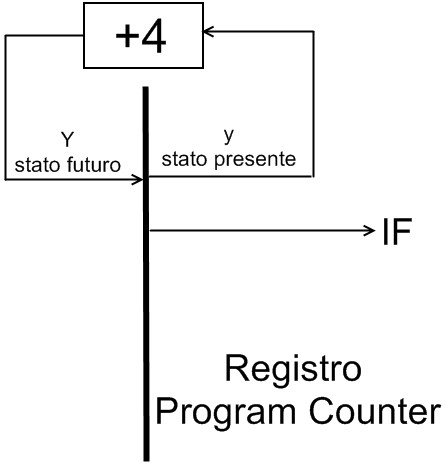
\includegraphics[width=0.35\columnwidth]{img/plusFour}
\caption{Usuale calcolo del PC: come ci regoliamo nel caso di predizione di salto?}
\label{fig:plusFour}
\end{figure}

Ogni volta che si abbisogna di un dato si controlla ispezionando la colonna \textit{nome} della nostra memoria: se trovo l'informazione cercata ho una \textit{hit}, altrimenti una \textit{miss}.
Volendo costruire questo tipo di memoria affinché sia superveloce bisogna inserire un comparatore per ogni elemento della tabella, in modo da confrontare il nome cercato con tutte le possibili \textit{entry} (memoria \textit{fully associative)}: facendo l'OR logico di tutte le uscite dei comparatori (1 = presenza, 0 = assenza) siamo in grado di ottenere in segnale di MISS negato (o di HIT). Con questa scelta bastano pochissimi clock\footnote{Almeno uno, ma non tanti di più!} e la velocità è nettamente superiore a quella che si ha con un \textit{loop} software.

\begin{figure}[!h]
\centering
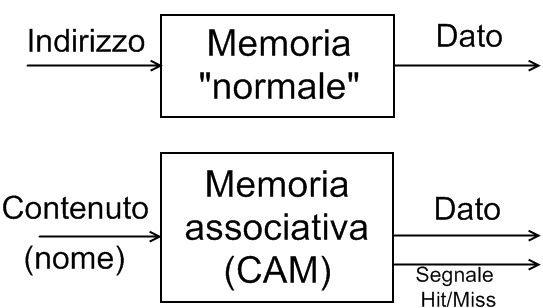
\includegraphics[width=0.4\columnwidth]{img/memVScam}
\caption{Memorie associative e memorie ordinarie (RAM, \textit{Random Access Memory})}
\label{fig:memVScam}
\end{figure}

A questo punto basta memorizzare, come coppie nome/valore, i PC futuri (cioè predetti) assieme al loro identificatore ed ecco che abbiamo ottenuto una velocissima struttura di predizione.
Grazie all'apparato di figura \ref{fig:plusFourModified} siamo quindi in grado di saltare, in base ad una corretta (\textit{hit}) o errata (\textit{miss}) predizione, al PC corretto. Il multiplexer in figura è un multiplexer a 32 bit e 2 vie (realizzato con 32 multiplexer da 1 bit).

\begin{figure}[!h]
\centering
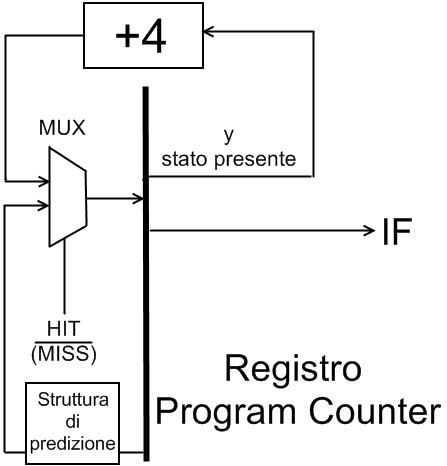
\includegraphics[width=0.4\columnwidth]{img/plusFourModified}
\caption{Versione modificata dell'apparato di selezione del PC}
\label{fig:plusFourModified}
\end{figure}

Come viene aggiornata la tabella? Il programma, quando scopre l'esistenza di una \textit{branch}, inserisce nella tabella il PC al quale si potrà saltare (se il salto avverrà) definisce una coppia nome/valore. La tabella (memoria associativa) verrà quindi esaminata ogniqualvolta si presenterà un'istruzione di salto: se sarà la prima volta che si effettua tale istruzione\footnote{CAM vuota: si cerca comunque di fare una predizione statica, non potendo fare diversamente.}, avremo obbligatoriamente una \textit{miss} e inseriremo il PC a cui si sarebbe dovuti saltare all'interno della CAM. Le volte successive, invece, saremo più fortunati se in tabella sarà ancora presente la \textit{entry} relativa a quel tipo di salto (cosa che molto plausibile che avvenga, vista l'esistenza del cosiddetto \textit{principio di località temporale}, il quale in soldoni recita che, effettuando spesso una certa istruzione o attingendo spesso a un dato, è molto probabile una futura intensa riutilizzazione di quell'istruzione/dato\footnote{"'Se faccio una cosa la riferò, se smetto di farla non la farò presumibilmente più'". (cit.)} in tempi relativamente brevi\footnote{Si pensi, ad esempio, ad un loop.}).

\section{Memorie associative e traduzione degli indirizzi}
\label{sec:associativeIndirizzi}

La CAM (che, organizzata come descritto, è detta anche \textit{Branch Tagged Buffer}) "'accelera la CPU'" conservando al suo interno i PC futuri che andranno quasi-sicuramente bene se vige il regime di località temporale (come effettivamente accade).
Nel caso la tabella sia piena o parzialmente piena, la cosa più logica è quella di cancellare l'istruzione non usata da più tempo: a far questo ci pensa un particolare algoritmo di sostituzione facente uso di una lista, detta \textit{list recently used}, in grado di discriminare le informazioni accedute più di recente. Inoltre, si cerca di mantenere gelosamente in tabella le istruzioni con il più basso parametro di \textit{miss-rate}\footnote{Calcolato come rapporta fra numero di \textit{miss} e numero di accessi.} (o il più alto \textit{hit-rate}), sacrificando piuttosto quelle con un più alto numero di \textit{miss}.

Questa tecnica viene utilizzata anche per la traduzione degli indirizzi delle istruzioni in \textit{cache} (indirizzati con 15 bit\footnote{Supponendo che la \textit{cache} sia di 32 KB.}) e quelle in memoria centrale (indirizzate con 32 bit\footnote{Supponendo che la memoria centrale sia di 4 GB.}). 
\[
IF_{32} \Rightarrow IC_{15}
\]
Stessa cosa può essere fatta tra memoria centrale e memoria virtuale\footnote{In informatica, la memoria virtuale è un tipo di memoria che ha la stessa funzione della RAM, ma viene usata solo se quest'ultima è piena e non riesce più a contenere informazioni; questo risultato si raggiunge utilizzando spazio di memoria secondaria su altri dispositivi, di solito le unità a disco (purtroppo più lente). La memoria centrale fisicamente presente diventa quindi la parte effettivamente utilizzata di quella virtuale, più grande: questo stratagemma è utile in virtù del principio di località e riuso dell'esecuzione dei programmi.}

\section{\textit{Pipeline} e linguaggi \textit{memory-register}}
\label{sec:pipelineMemoryRegister}

Quasi tutti gli esempi fatti fin'ora fanno riferimento alla struttura del DLX (registro-registro): come viene però implementata la \textit{pipeline} nei sistemi memoria-registro, con particolare riferimento al calcolo degli indirizzi (il quale dev'essere effettuato in maniera assolutamente trasparente)?

Per esemplificare consideriamo un linguaggio di tipo Intel e l'istruzione:
\begin{verbatim}
ADD     DS:[BX+DI], ALFA, AL
\end{verbatim}
L'indirizzo logico dell'operando sul quale andiamo ad agire è costituito dal binomio (base, offset) = $(DS, BX + DI + ALFA)$.
L'indirizzo fisico sarà invece pari a: $DS \cdot 2^4 + BX + DI + ALFA$ (dove il $2^4$ è dovuto al fatto che l'indirizzo in DS [\textit{Data Segment}] ha i quattro bit meno significativi sempre posti a 0 in quanto indirizziamo blocchi di $2^4$ byte sulla memoria fisica di 1 MB).
Dunque il calcolo dell'indirizzo fisico richiede di effettuare tre somme, terminate le quali l'indirizzo viene schiaffato\footnote{Termine tecnico.} sul bus degli indirizzi ($BA19,\ldots,BA0$).

Come effettuare queste operazioni in una \textit{pipeline}? Una prima modifica alla \textit{pipeline} che conosciamo, consiste nell'introduzione di un nuovo stadio a valle di ID destinato a calcolare l'indirizzo dell'operando in memoria (AG,\textit{ Address Generator}, o ID2, nome adottato da Intel per il Pentium): a tal fine lo stadio AG deve disporre di tre sommatori veloci in cascata.
Una seconda modifica consiste nel riunire i due stadi EX e MEM in un unico stadio (multiciclo) in cui sono localizzate la ALU e la cache dei dati. Questo stadio detto EX-MEM imporrà alle istruzioni la permanenza di un numero di colpi di clock variabile in funzione dell'istruzione eseguita: la valutazione viene effettuata considerando quante operazioni elementari di ALU o di accesso alla memoria devono essere effettuate per eseguire correttamente l'istruzione considerata\footnote{Esempi:
\begin{itemize}
\item  le istruzioni di trasferimento dati (con \textit{hit} in \textit{cache} dati) restano in EX-MEM un
periodo di clock;
\item  le istruzioni di ALU con un operando in memoria (\textit{hit}) e risultato su registro restano in
EX-MEM due clock (uno per leggere l'operando e uno per calcolare il risultato;
\item le istruzioni di ALU con un operando in memoria (\textit{hit}) e risultato in memoria restano
in EX-MEM tre clock (uno per leggere l'operando, uno per calcolare il risultato e uno
per aggiornare la memoria).
\end{itemize}
}

\begin{figure}[!h]
\centering
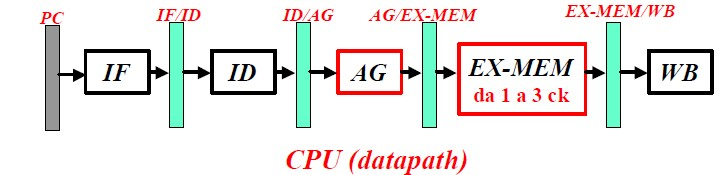
\includegraphics[width=0.8\columnwidth]{img/intelDataPath}
\caption{Modifiche alla \textit{pipeline} per sistemi Intel}
\label{fig:intelDataPath}
\end{figure}

Rispetto al DLX le cose vanno leggermente meglio grazie alla migliore densità del codice (il linguaggio Intel è CISC): il tutto mantenendo un CPI medio piuttosto piccolo (caratteristica dei sistemi RISC).


Come ci comportiamo con le istruzioni come quelle di \textit{push all}, in cui è necessario tradurre un'unica istruzione di linguaggio-macchina in almeno una decina di istruzioni elementari? La scelta effettuata è quella di bloccare la \textit{fetch} mentre viene alimentata la \textit{pipeline} con istruzioni elementari.

\subsection{Architetture superscalari}
\label{sec:superscalarArchitectures}

\begin{figure}[!h]
\centering
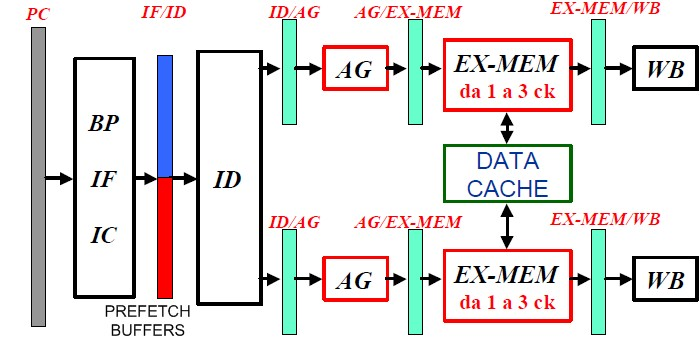
\includegraphics[width=0.9\columnwidth]{img/superscalare}
\caption{Schema di un'architettura superscalare (Pentium)}
\label{fig:superscalare}
\end{figure}

E se volessimo avere un parametro IPC (\textit{Instructions Per Clock} $= 1/CPI$) maggiore di 1? Dobbiamo ricorrere ad architetture cosiddette \textit{superscalari} (ad es. \textit{Pentium} IA32): si definisce infatti \textit{superscalare} una architettura che può attivare più di una istruzione nello stesso periodo di clock.
Nelle architetture superscalari lo stadio IF preleva in parallelo da IC frammenti di codice di
lunghezza maggiore o uguale a due istruzioni [nel Pentium: blocchi di codice di dimensione costante (32 byte) passati a ID attraverso un \textit{prefetch buffer}]; nello stadio AG vengono calcolati gli indirizzi degli operandi in memoria: le istruzioni complesse (istruzioni CISC descritte con microcodice) sfruttano le due \textit{pipeline} per una maggiore velocità.

In caso di istruzioni di trasferimento del controllo l'indirizzo di \textit{fetch} viene generato
dalla logica di predizione (ad esempio grazie alle memorie associative); successivamente IF preleverà codice anche dall'indirizzo associato alla situazione di \textit{misprediction} e lo appoggerà sull'altro \textit{prefetch buffer} Le istruzioni da decodificare si prelevano dallo stesso \textit{prefetch buffer} finché non si
verifica un errore di predizione, che viene rilevato alla fine della \textit{pipeline}. In caso di errore di predizione le \textit{pipeline} vengono svuotate e cambia il \textit{prefetch buffer} da cui si preleva il codice da eseguire: il \textit{prefetch buffer} è quindi in grado di ridurre il numero di stalli in caso di \textit{misprediction}.

ID riconosce due istruzioni consecutive sul \textit{prefetch buffer}, verifica che le due istruzioni
possano essere eseguite in parallelo e in tal caso le passa allo stadio a valle insieme al
contenuto dei registri operandi delle istruzioni. Se le due istruzioni non possono essere eseguite in parallelo (\textit{pairing rules} non soddisfatte), allora viene passata a valle una sola istruzione. Dallo stadio AG in poi le istruzioni che si trovano in stadi omonimi avanzano nella \textit{pipeline} insieme; se una istruzione stalla, stallerà anche l'altra, e stallano anche tutte le istruzioni che si trovano negli stadi a monte (\textit{pipeline} \textit{bloccanti}), dunque le istruzioni non possono sorpassarsi nella \textit{pipeline} (esecuzione e
completamento \textit{in ordine}).

Infine, al fine di ridurre gli stalli ogni \textit{pipeline} dispone, in EX-MEM, di un buffer di scrittura su cui
depositare indirizzi e dati da inviare alla memoria in caso di \textit{miss} in scrittura.
